\begin{figure}[h!]
	\centering
	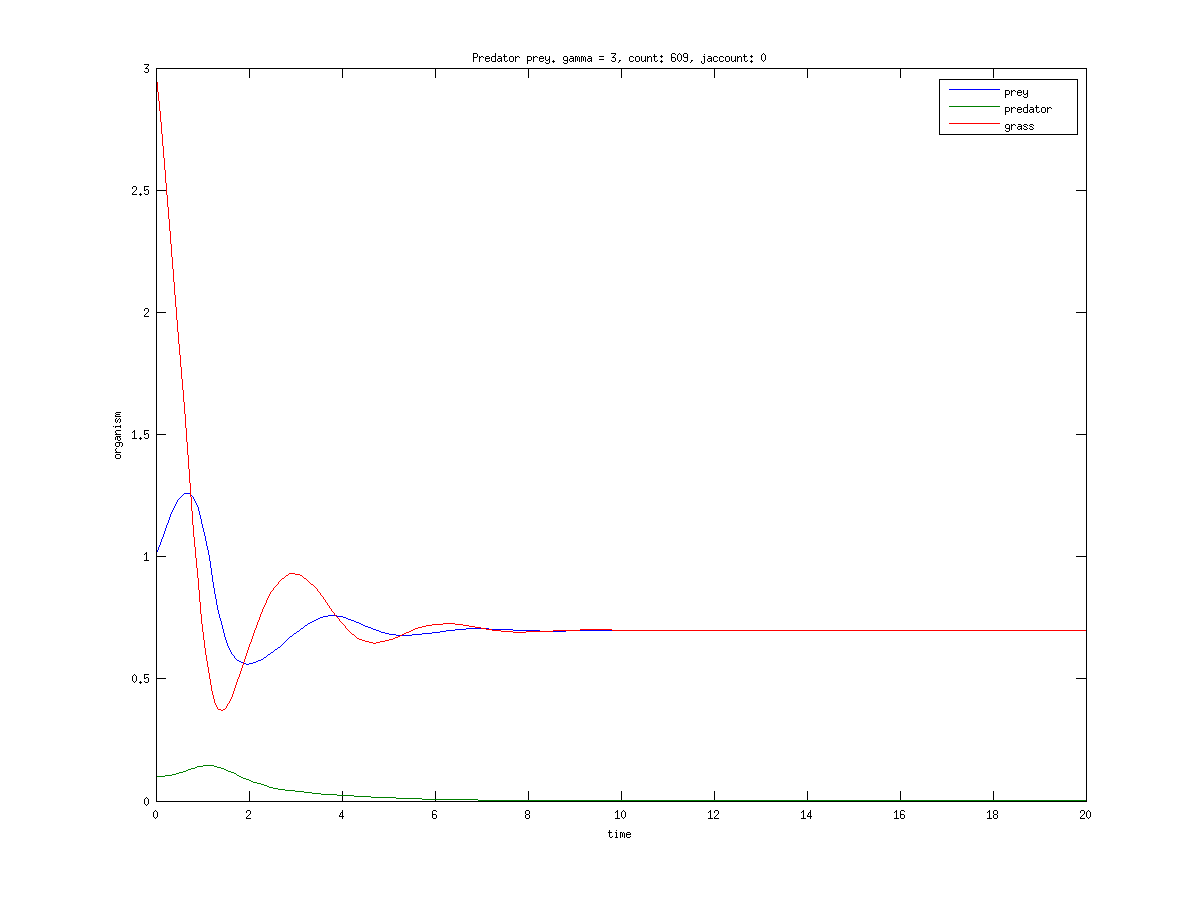
\includegraphics[width=0.8\textwidth]{img/exc3_3}
	\caption{Predator prey. Solved using rkf45 with parameter $\gamma = 3$.}
	\label{fig:exc3_3}
\end{figure}


\begin{figure}[h!]
	\centering
	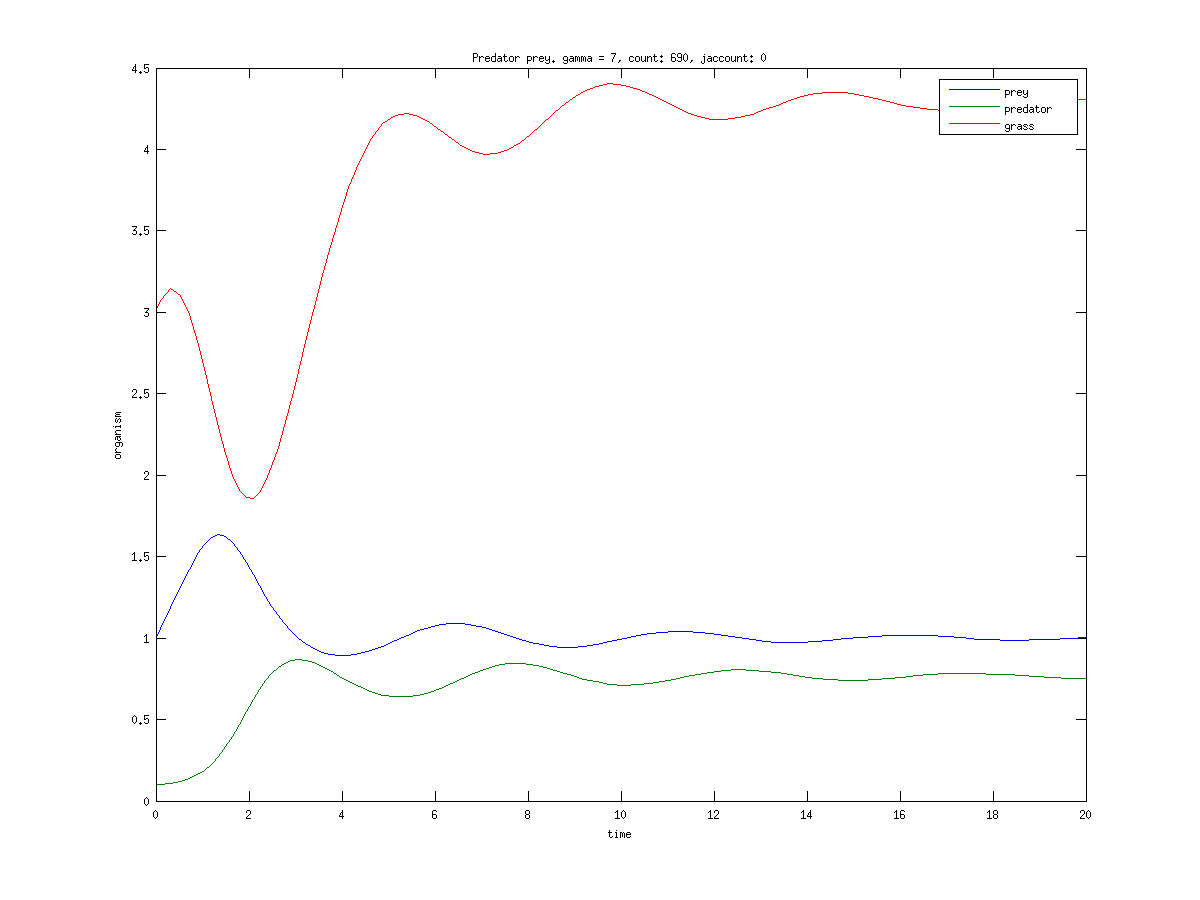
\includegraphics[width=0.8\textwidth]{img/exc3_7}
	\caption{Predator prey. Solved using rkf45 with parameter $\gamma = 7$.}
	\label{fig:exc3_7}
\end{figure}

Lower gamma reaches steady state faster. Higher gamma increases predator population more than prey. At gamme=3 the predator population actually dies out.
This is using the extra term with gmax.

If we leave out the gmax term in the grass equation. The grass will grow without bounds for large enough gamma, see fig. \ref{fig:exc3_7_gmax}

\begin{figure}[h!]
	\centering
	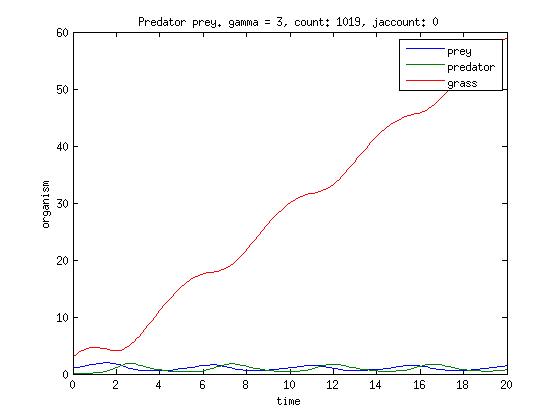
\includegraphics[width=0.8\textwidth]{img/exc3_7_gmax}
	\caption{Predator prey. Solved using rkf45 with parameter $\gamma = 7$ but without gmax term in the grass equation.}
	\label{fig:exc3_7_gmax}
\end{figure}